%=====================================================================
%  Lattice Multiplication  --  from area model to grid to lattice
%  Beamer / TikZ.  Compile with pdflatex (twice).
%=====================================================================
\documentclass[10pt,aspectratio=169]{beamer}

\usepackage[T1]{fontenc}
%\usepackage{lmodern} % not installed here; safe to re-enable locally
\usepackage{amsmath,amssymb}
\usepackage{array,colortbl}
\usepackage{tikz}
\usetikzlibrary{calc,positioning,arrows.meta,decorations.pathreplacing}

\usetheme{default}
\usecolortheme{default}
\setbeamertemplate{navigation symbols}{}
\setbeamertemplate{itemize items}[circle]

%--------------------------------------------------- colours
\definecolor{mmblue}{RGB}{28,77,120}
\definecolor{mmred}{RGB}{176,42,55}
\definecolor{mmgreen}{RGB}{35,110,75}
\definecolor{mmgrey}{RGB}{120,120,120}
\definecolor{bandA}{RGB}{255,232,200}   % units      diagonal
\definecolor{bandB}{RGB}{212,233,246}   % tens       diagonal
\definecolor{bandC}{RGB}{225,243,220}   % hundreds   diagonal
\definecolor{bandD}{RGB}{238,225,243}   % thousands  diagonal

\setbeamercolor{frametitle}{fg=white,bg=mmblue}
\setbeamercolor{title}{fg=mmblue}
\setbeamercolor{structure}{fg=mmblue}
\setbeamerfont{frametitle}{series=\bfseries}
\setbeamertemplate{frametitle}{%
  \vspace*{2pt}\hspace*{6pt}\insertframetitle\vspace*{3pt}}

%--------------------------------------------------- answer overlay
% If your own preamble already defines these, yours are used instead.
\providecommand{\ablank}[1]{\uncover<2->{\textcolor{mmred}{#1}}}
\providecommand{\ashow}[1]{\textcolor{mmred}{#1}}

%--------------------------------------------------- lattice toolkit
\tikzset{
  cellline/.style={draw=mmblue,line width=0.7pt},
  diagline/.style={draw=mmblue!60,line width=0.6pt},
  headfont/.style={font=\bfseries},
}

% \lgrid{cols}{rows} : boxes + diagonals
\newcommand{\lgrid}[2]{%
  \foreach \c in {1,...,#1}{%
    \foreach \r in {1,...,#2}{%
      \draw[cellline] ({\c-1},{-\r+1}) rectangle ({\c},{-\r});
      \draw[diagline] ({\c},{-\r+1}) -- ({\c-1},{-\r});}}%
}

% \lband{cols}{rows}{a}{colour} : shade the strip a <= x-y <= a+1
\newcommand{\lband}[4]{%
  \begin{scope}
    \clip (0,0) rectangle ({#1},{-#2});
    \fill[#4] ({#3},0) -- ({#3+1},0) -- ({#3-7},-8) -- ({#3-8},-8) -- cycle;
  \end{scope}%
}

% \ldiag{cols}{rows}{a}{colour} : draw the diagonal line x-y = a, extended
\newcommand{\ldiag}[4]{%
  \begin{scope}
    \clip ({-0.6},0.0) rectangle ({#1},{-#2-0.6});
    \draw[#4,line width=1.4pt] ({#3+1},1) -- ({#3-8},-8);
  \end{scope}%
}

% \ltop{col}{digit}  column heading
\newcommand{\ltop}[2]{\node[headfont] at ({#1-0.5},{0.32}) {#2};}
% \lside{cols}{row}{digit}  row heading on the right
\newcommand{\lside}[3]{\node[headfont] at ({#1+0.35},{-#2+0.5}) {#3};}
% \lcell{col}{row}{tens}{units}
\newcommand{\lcell}[4]{%
  \node at ({#1-0.72},{-#2+0.70}) {\small #3};
  \node at ({#1-0.28},{-#2+0.30}) {\small #4};}
% \lleft{row}{digit}  answer digit at left edge
\newcommand{\lleft}[2]{\node[mmred,font=\bfseries] at ({-0.42},{-#1+0.5}) {#2};}
% \lbot{cols}{rows}{col}{digit} answer digit under the bottom edge
\newcommand{\lbot}[4]{\node[mmred,font=\bfseries] at ({#3-0.5},{-#2-0.42}) {#4};}

%--------------------------------------------------- misc
\newcommand{\hl}[1]{\textcolor{mmred}{#1}}
\newcommand{\gd}[1]{\textcolor{mmgreen}{#1}}
\renewcommand{\arraystretch}{1.35}

\title{Lattice Multiplication}
\subtitle{From rectangles, to grids, to diagonals}
\author{}
\date{}

\begin{document}

%=====================================================================
\begin{frame}[plain]
  \vfill
  \centering
  {\Huge\bfseries\color{mmblue} Lattice Multiplication}\\[4pt]
  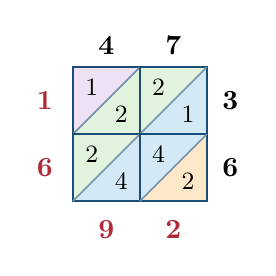
\begin{tikzpicture}[scale=0.85]
    \lband{2}{2}{3}{bandA}\lband{2}{2}{2}{bandB}
    \lband{2}{2}{1}{bandC}\lband{2}{2}{0}{bandD}
    \lgrid{2}{2}
    \ltop{1}{4}\ltop{2}{7}\lside{2}{1}{3}\lside{2}{2}{6}
    \lcell{1}{1}{1}{2}\lcell{2}{1}{2}{1}
    \lcell{1}{2}{2}{4}\lcell{2}{2}{4}{2}
    \lleft{1}{1}\lleft{2}{6}\lbot{2}{2}{1}{9}\lbot{2}{2}{2}{2}
  \end{tikzpicture}
  \vfill
\end{frame}

%=====================================================================
\begin{frame}{Where we are going}
  \begin{columns}[T]
    \begin{column}{0.33\textwidth}
      \centering
      {\color{mmblue}\bfseries 1. Area}\\[6pt]
      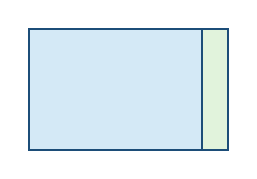
\begin{tikzpicture}[scale=0.11]
        \fill[bandB] (0,0) rectangle (20,14);
        \fill[bandC] (20,0) rectangle (23,14);
        \draw[mmblue,thick] (0,0) rectangle (23,14);
        \draw[mmblue] (20,0) -- (20,14);
      \end{tikzpicture}\\[6pt]
      {\footnotesize Multiplying is finding the area of a rectangle.}
    \end{column}
    \begin{column}{0.33\textwidth}
      \centering
      {\color{mmblue}\bfseries 2. Grid method}\\[6pt]
      {\footnotesize
      \begin{tabular}{|c|c|c|}\hline
        $\times$ & $20$ & $3$\\\hline
        $10$ & $200$ & $30$\\\hline
        $4$ & $80$ & $12$\\\hline
      \end{tabular}}\\[6pt]
      {\footnotesize The rectangle written as a table. Every zero shown.}
    \end{column}
    \begin{column}{0.33\textwidth}
      \centering
      {\color{mmblue}\bfseries 3. Lattice}\\[6pt]
      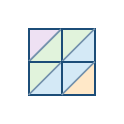
\begin{tikzpicture}[scale=0.42]
        \lband{2}{2}{3}{bandA}\lband{2}{2}{2}{bandB}
        \lband{2}{2}{1}{bandC}\lband{2}{2}{0}{bandD}
        \lgrid{2}{2}
      \end{tikzpicture}\\[6pt]
      {\footnotesize The same products, with the diagonals doing the place value.}
    \end{column}
  \end{columns}
  \vspace{10pt}
\end{frame}

%=====================================================================
\begin{frame}{Multiplication is area}
  \begin{columns}[c]
    \begin{column}{0.5\textwidth}
      \centering
      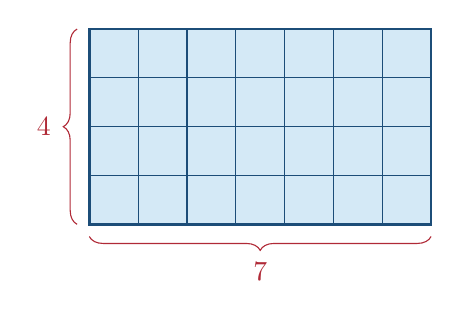
\begin{tikzpicture}[scale=0.62]
        \fill[bandB] (0,0) rectangle (7,4);
        \draw[mmblue,step=1] (0,0) grid (7,4);
        \draw[mmblue,line width=1pt] (0,0) rectangle (7,4);
        \draw[decorate,decoration={brace,amplitude=5pt,mirror},mmred]
              (0,-0.25) -- (7,-0.25) node[midway,below=6pt]{$7$};
        \draw[decorate,decoration={brace,amplitude=5pt},mmred]
              (-0.25,0) -- (-0.25,4) node[midway,left=6pt]{$4$};
      \end{tikzpicture}
    \end{column}
    \begin{column}{0.5\textwidth}
      \begin{itemize}
        \item A rectangle $7$ wide and $4$ tall.
        \item Count the squares: $7 \times 4 = 28$.
        \item[]
        \item {\color{mmblue}\bfseries Every multiplication question can be represented as a rectangle.}
      \end{itemize}
    \end{column}
  \end{columns}
\end{frame}

%=====================================================================
\begin{frame}{Chopping the rectangle up}
  \begin{center}
    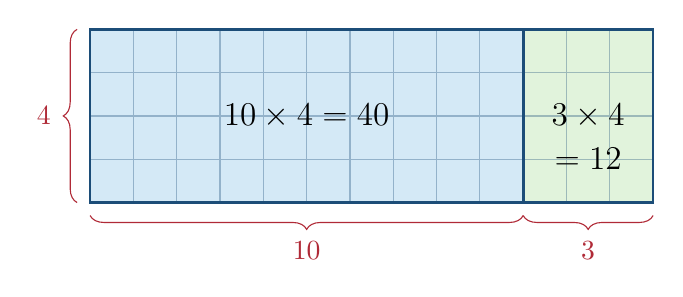
\begin{tikzpicture}[scale=0.55]
      \fill[bandB] (0,0) rectangle (10,4);
      \fill[bandC] (10,0) rectangle (13,4);
      \draw[mmblue,step=1,opacity=0.35] (0,0) grid (13,4);
      \draw[mmblue,line width=1pt] (0,0) rectangle (13,4);
      \draw[mmblue,line width=1.2pt] (10,0) -- (10,4);
      \node at (5,2) {\large $10\times 4 = 40$};
      \node at (11.5,2) {\large $3\times 4$};
      \node at (11.5,1) {\large $=12$};
      \draw[decorate,decoration={brace,amplitude=5pt,mirror},mmred]
            (0,-0.3) -- (10,-0.3) node[midway,below=6pt]{$10$};
      \draw[decorate,decoration={brace,amplitude=5pt,mirror},mmred]
            (10,-0.3) -- (13,-0.3) node[midway,below=6pt]{$3$};
      \draw[decorate,decoration={brace,amplitude=5pt},mmred]
            (-0.3,0) -- (-0.3,4) node[midway,left=6pt]{$4$};
    \end{tikzpicture}
  \end{center}
  \vspace{-4pt}
  \begin{center}
    \large $13 \times 4 \;=\; (10\times 4) + (3\times 4) \;=\; 40 + 12 \;=\; \hl{52}$
  \end{center}
  \vspace{4pt}
  {\color{mmgrey}\small We split $13$ into the parts we can actually multiply in our
   heads: its \emph{tens} and its \emph{units}.}
\end{frame}

%=====================================================================
\begin{frame}{Two digits by two digits: four pieces}
  \begin{center}
    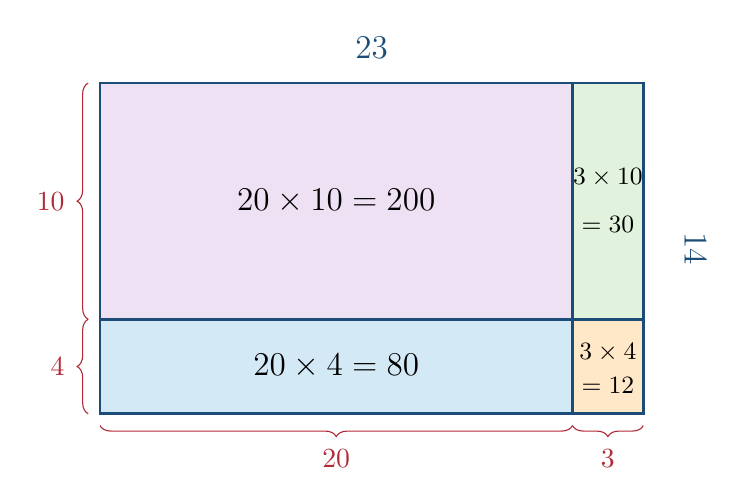
\begin{tikzpicture}[scale=0.30]
      \fill[bandD] (0,4) rectangle (20,14);
      \fill[bandC] (20,4) rectangle (23,14);
      \fill[bandB] (0,0) rectangle (20,4);
      \fill[bandA] (20,0) rectangle (23,4);
      \draw[mmblue,line width=1pt] (0,0) rectangle (23,14);
      \draw[mmblue,line width=1.2pt] (20,0) -- (20,14);
      \draw[mmblue,line width=1.2pt] (0,4) -- (23,4);
      \node at (10,9)   {\large $20\times 10 = 200$};
      \node at (21.5,10) {\small $3\times 10$};
      \node at (21.5,8)  {\small $=30$};
      \node at (10,2)   {\large $20\times 4 = 80$};
      \node at (21.5,2.6) {\small $3\times4$};
      \node at (21.5,1.2) {\small $=12$};
      \draw[decorate,decoration={brace,amplitude=4pt,mirror},mmred]
            (0,-0.5) -- (20,-0.5) node[midway,below=5pt]{$20$};
      \draw[decorate,decoration={brace,amplitude=4pt,mirror},mmred]
            (20,-0.5) -- (23,-0.5) node[midway,below=5pt]{$3$};
      \draw[decorate,decoration={brace,amplitude=4pt},mmred]
            (-0.5,4) -- (-0.5,14) node[midway,left=5pt]{$10$};
      \draw[decorate,decoration={brace,amplitude=4pt},mmred]
            (-0.5,0) -- (-0.5,4) node[midway,left=5pt]{$4$};
      \node[mmblue] at (11.5,15.5) {\large\bfseries $23$};
      \node[mmblue,rotate=-90] at (25.2,7) {\large\bfseries $14$};
    \end{tikzpicture}
  \end{center}
  \vspace{-2pt}
  \begin{center}
    \large $23\times 14 \;=\; 200 + 30 + 80 + 12 \;=\; \hl{322}$
  \end{center}
\end{frame}

%=====================================================================
\begin{frame}{The same rectangle, written as a grid}
  \begin{columns}[c]
    \begin{column}{0.46\textwidth}
      \centering
      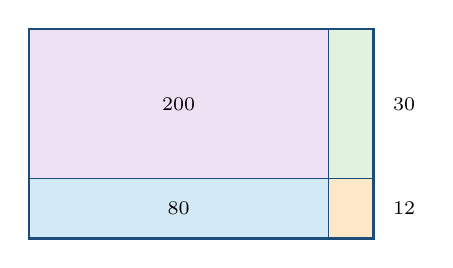
\begin{tikzpicture}[scale=0.19]
        \fill[bandD] (0,4) rectangle (20,14);
        \fill[bandC] (20,4) rectangle (23,14);
        \fill[bandB] (0,0) rectangle (20,4);
        \fill[bandA] (20,0) rectangle (23,4);
        \draw[mmblue,line width=1pt] (0,0) rectangle (23,14);
        \draw[mmblue] (20,0) -- (20,14);
        \draw[mmblue] (0,4) -- (23,4);
        \node[font=\scriptsize] at (10,9) {$200$};
        \node[font=\scriptsize] at (10,2) {$80$};
        \node[font=\scriptsize,right=1pt] at (23.5,9) {$30$};
        \node[font=\scriptsize,right=1pt] at (23.5,2) {$12$};
      \end{tikzpicture}
    \end{column}
    \begin{column}{0.10\textwidth}
      \centering{\Huge\color{mmblue}$\Rightarrow$}
    \end{column}
    \begin{column}{0.42\textwidth}
      \centering
      \begin{tabular}{|c|c|c|}\hline
        \bfseries $\times$ & \bfseries $20$ & \bfseries $3$\\\hline
        \bfseries $10$ & \cellcolor{white}$200$ & $30$\\\hline
        \bfseries $4$ & $80$ & $12$\\\hline
      \end{tabular}\\[10pt]
      {\small $200+30+80+12 = \hl{322}$}
    \end{column}
  \end{columns}
  \vspace{8pt}
  \begin{itemize}
    \item The grid is like the picture, but not drawn to scale.
  \end{itemize}
\end{frame}

%=====================================================================
\begin{frame}{Keep every zero}
  \begin{center}
    \begin{tabular}{|c|c|c|}\hline
      \bfseries $\times$ & \bfseries $40$ & \bfseries $7$\\\hline
      \bfseries $30$ & $1200$ & $210$\\\hline
      \bfseries $6$  & $240$  & $42$\\\hline
    \end{tabular}
    \hspace{18pt}
    \begin{minipage}{0.42\textwidth}
      \begin{align*}
        4\times 3 &= 12 &&\text{so } \hl{40}\times \hl{30} = \hl{1200}\\
        4\times 6 &= 24 &&\text{so } \hl{40}\times 6 = \hl{240}\\
        7\times 3 &= 21 &&\text{so } 7\times \hl{30} = \hl{210}\\
        7\times 6 &= 42 &&\text{so } 7\times 6 = 42
      \end{align*}
    \end{minipage}
  \end{center}
  \vspace{4pt}
  \begin{center}
    \large $1200+240+210+42 = \hl{1692}$, \quad so $47\times 36 = \hl{1692}$
  \end{center}
  \vspace{4pt}
\end{frame}

%=====================================================================
\begin{frame}{Your turn: grid method}
  \begin{center}
    \begin{tabular}{lll}
      \textbf{(a)} $34\times 12 = \ablank{408}$ &\quad
      \textbf{(b)} $26\times 45 = \ablank{1170}$ &\quad
      \textbf{(c)} $53\times 27 = \ablank{1431}$\\[10pt]
      \textbf{(d)} $18\times 63 = \ablank{1134}$ &\quad
      \textbf{(e)} $72\times 84 = \ablank{6048}$ &\quad
      \textbf{(f)} $95\times 48 = \ablank{4560}$
    \end{tabular}
  \end{center}
  \vspace{10pt}
  \begin{center}
    \begin{tabular}{|c|c|c|}\hline
      \bfseries $\times$ & & \\\hline
      & & \\\hline
      & & \\\hline
    \end{tabular}
    \hspace{20pt}
    \begin{minipage}{0.45\textwidth}
      \small \textbf{Challenge.} $124 \times 36$. How many boxes does your
      grid need now, and why? \\[4pt]
      Answer: \ablank{$3\times 2 = 6$ boxes, one for each pair of place values; $124\times 36 = 4464$}
    \end{minipage}
  \end{center}
\end{frame}

%=====================================================================
\begin{frame}{The problem with the grid}
  \begin{center}
    \begin{tabular}{|c|c|c|c|}\hline
      \bfseries $\times$ & \bfseries $300$ & \bfseries $40$ & \bfseries $7$\\\hline
      \bfseries $600$ & $180000$ & $24000$ & $4200$\\\hline
      \bfseries $50$  & $15000$  & $2000$  & $350$\\\hline
      \bfseries $8$   & $2400$   & $320$   & $56$\\\hline
    \end{tabular}
  \end{center}
  \vspace{8pt}
  \begin{itemize}
    \item The method is fine for bigger numbers... 
    \item But it is a lot of writing long numbers
    \item[]
    \item {\color{mmblue}\bfseries The lattice keeps the same nine products but
          writes only the digits} --- and uses \emph{diagonals} instead of zeros to
          keep track of place value.
  \end{itemize}
\end{frame}

%=====================================================================
\begin{frame}{Building a lattice: step 1, draw it}
  \begin{columns}[c]
    \begin{column}{0.45\textwidth}
      \centering
      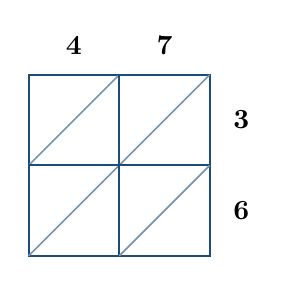
\begin{tikzpicture}[scale=1.15]
        \lgrid{2}{2}
        \ltop{1}{4}\ltop{2}{7}\lside{2}{1}{3}\lside{2}{2}{6}
      \end{tikzpicture}
    \end{column}
    \begin{column}{0.55\textwidth}
      \begin{itemize}
        \item $47 \times 36$.
        \item One \emph{column} for each digit of $47$, written across the top.
        \item One \emph{row} for each digit of $36$, written down the right.
        \item Draw a diagonal in every cell, running from
              {\color{mmblue}top-right down to bottom-left}.
      \end{itemize}
    \end{column}
  \end{columns}
\end{frame}

%=====================================================================
\begin{frame}{Step 2: fill every cell with a times-table fact}
  \begin{columns}[c]
    \begin{column}{0.45\textwidth}
      \centering
      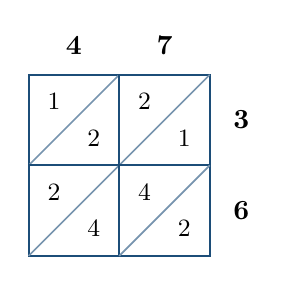
\begin{tikzpicture}[scale=1.15]
        \lgrid{2}{2}
        \ltop{1}{4}\ltop{2}{7}\lside{2}{1}{3}\lside{2}{2}{6}
        \lcell{1}{1}{1}{2}\lcell{2}{1}{2}{1}
        \lcell{1}{2}{2}{4}\lcell{2}{2}{4}{2}
      \end{tikzpicture}
    \end{column}
    \begin{column}{0.55\textwidth}
      \begin{itemize}
        \item Multiply each of the combinations of digits in the relevant cell.
        \item \textbf{Tens} go in the upper-left triangle, \textbf{units} in the
              lower-right.
        \item[]
      \end{itemize}
      \begin{center}
        \small
        \begin{tabular}{ll}
          $4\times3=12$ & $\rightarrow$ \;$\boxed{1}\,/\,\boxed{2}$\\
          $7\times3=21$ & $\rightarrow$ \;$\boxed{2}\,/\,\boxed{1}$\\
          $4\times6=24$ & $\rightarrow$ \;$\boxed{2}\,/\,\boxed{4}$\\
          $7\times6=42$ & $\rightarrow$ \;$\boxed{4}\,/\,\boxed{2}$
        \end{tabular}
      \end{center}
      \vspace{4pt}
      {\color{mmgrey}\small A one-digit answer such as $3\times2=6$ is written $0/6$.}
    \end{column}
  \end{columns}
\end{frame}

%=====================================================================
\begin{frame}{Step 3: add along the diagonals}
  \begin{columns}[c]
    \begin{column}{0.48\textwidth}
      \centering
      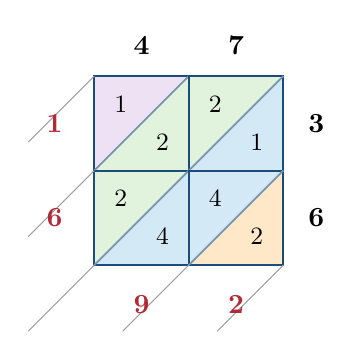
\begin{tikzpicture}[scale=1.2]
        \lband{2}{2}{3}{bandA}\lband{2}{2}{2}{bandB}
        \lband{2}{2}{1}{bandC}\lband{2}{2}{0}{bandD}
        \lgrid{2}{2}
        % let each diagonal run out of the lattice to its landing spot
        \draw[mmgrey!70] (0,0) -- (-0.7,-0.7);
        \draw[mmgrey!70] (0,-1) -- (-0.7,-1.7);
        \draw[mmgrey!70] (0,-2) -- (-0.7,-2.7);
        \draw[mmgrey!70] (1,-2) -- (0.3,-2.7);
        \draw[mmgrey!70] (2,-2) -- (1.3,-2.7);
        \ltop{1}{4}\ltop{2}{7}\lside{2}{1}{3}\lside{2}{2}{6}
        \lcell{1}{1}{1}{2}\lcell{2}{1}{2}{1}
        \lcell{1}{2}{2}{4}\lcell{2}{2}{4}{2}
        \lleft{1}{1}\lleft{2}{6}
        \lbot{2}{2}{1}{9}\lbot{2}{2}{2}{2}
      \end{tikzpicture}
    \end{column}
    \begin{column}{0.52\textwidth}
      Start at the bottom right and work up the strips.
      \begin{center}\small
      \begin{tabular}{lll}
        \cellcolor{bandA}units     & $2$            & $=\hl{2}$\\
        \cellcolor{bandB}tens      & $4+4+1$        & $=\hl{9}$\\
        \cellcolor{bandC}hundreds  & $2+2+2$        & $=\hl{6}$\\
        \cellcolor{bandD}thousands & $1$            & $=\hl{1}$\\
      \end{tabular}
      \end{center}
      \vspace{6pt}
      \begin{itemize}
        \item Each shaded strip is one \emph{place-value column}.
        \item Write each total just outside the lattice
      \end{itemize}
    \end{column}
  \end{columns}
\end{frame}

%=====================================================================
\begin{frame}{Step 4: read the answer down the left and along the bottom}
  \begin{columns}[c]
    \begin{column}{0.48\textwidth}
      \centering
      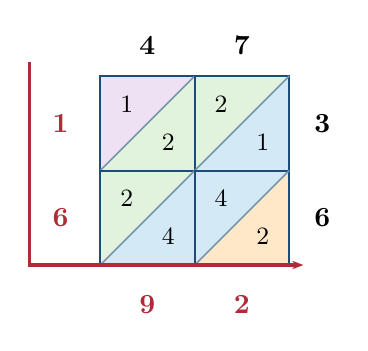
\begin{tikzpicture}[scale=1.2]
        \lband{2}{2}{3}{bandA}\lband{2}{2}{2}{bandB}
        \lband{2}{2}{1}{bandC}\lband{2}{2}{0}{bandD}
        \lgrid{2}{2}
        \ltop{1}{4}\ltop{2}{7}\lside{2}{1}{3}\lside{2}{2}{6}
        \lcell{1}{1}{1}{2}\lcell{2}{1}{2}{1}
        \lcell{1}{2}{2}{4}\lcell{2}{2}{4}{2}
        \lleft{1}{1}\lleft{2}{6}
        \lbot{2}{2}{1}{9}\lbot{2}{2}{2}{2}
        \draw[mmred,line width=1.2pt,-{Stealth[length=4pt]}]
              (-0.75,0.15) -- (-0.75,-2.0) -- (2.15,-2.0);
      \end{tikzpicture}
    \end{column}
    \begin{column}{0.52\textwidth}
      \begin{itemize}
        \item Read \textbf{down the left-hand side}, then \textbf{along the bottom}.
        \item $1,\;6,\;9,\;2$
        \item[]
        \item \Large $47 \times 36 = \hl{1692}$
      \end{itemize}
      \vspace{8pt}
      {\color{mmgrey}\small Compare with the grid method: $1200+240+210+42=1692$.
     its the same four products, the same answer --- but no long addition.}
    \end{column}
  \end{columns}
\end{frame}

%=====================================================================
\begin{frame}{What if a diagonal adds to more than 9?}
  \begin{columns}[c]
    \begin{column}{0.46\textwidth}
      \centering
      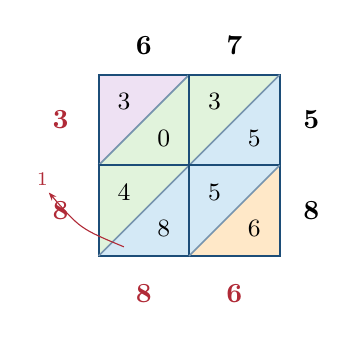
\begin{tikzpicture}[scale=1.15]
        \lband{2}{2}{3}{bandA}\lband{2}{2}{2}{bandB}
        \lband{2}{2}{1}{bandC}\lband{2}{2}{0}{bandD}
        \lgrid{2}{2}
        \ltop{1}{6}\ltop{2}{7}\lside{2}{1}{5}\lside{2}{2}{8}
        \lcell{1}{1}{3}{0}\lcell{2}{1}{3}{5}
        \lcell{1}{2}{4}{8}\lcell{2}{2}{5}{6}
        \lleft{1}{3}\lleft{2}{8}
        \lbot{2}{2}{1}{8}\lbot{2}{2}{2}{6}
        \node[mmred,font=\scriptsize] at (-0.62,-1.15) {$1$};
        \draw[mmred,-{Stealth[length=3pt]}] (0.28,-1.9) .. controls (-0.2,-1.7) .. (-0.55,-1.3);
      \end{tikzpicture}
    \end{column}
    \begin{column}{0.54\textwidth}
      \begin{center}\large $67 \times 58$\end{center}
      \begin{center}\small
      \begin{tabular}{lll}
        units     & $6$              & $=6$\\
        tens      & $5+8+5$          & $=18$ \;\hl{write 8, carry 1}\\
        hundreds  & $4+3+0+\hl{1}$   & $=8$\\
        thousands & $3$              & $=3$\\
      \end{tabular}
      \end{center}
      \vspace{6pt}
      \begin{itemize}
        \item If a strip totals $10$ or more, write down the units digit and
              \textbf{carry the tens into the next strip up-left}.
        \item Reading off: $3,\,8,\,8,\,6$ \quad$\Rightarrow$\quad
              $67\times 58 = \hl{3886}$
      \end{itemize}
      \vspace{2pt}
      {\color{mmgrey}\small Estimate: $70\times 60 = 4200$. \gd{\checkmark}}
    \end{column}
  \end{columns}
\end{frame}

%=====================================================================
\begin{frame}{Why do the diagonals work?}
  \begin{columns}[c]
    \begin{column}{0.44\textwidth}
      \centering
      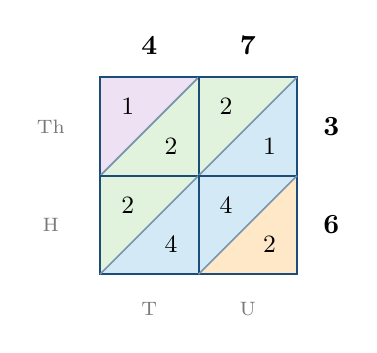
\begin{tikzpicture}[scale=1.25]
        \lband{2}{2}{3}{bandA}\lband{2}{2}{2}{bandB}
        \lband{2}{2}{1}{bandC}\lband{2}{2}{0}{bandD}
        \lgrid{2}{2}
        \ltop{1}{4}\ltop{2}{7}\lside{2}{1}{3}\lside{2}{2}{6}
        \lcell{1}{1}{1}{2}\lcell{2}{1}{2}{1}
        \lcell{1}{2}{2}{4}\lcell{2}{2}{4}{2}
        \node[font=\scriptsize,mmgrey] at (-0.5,-0.5) {Th};
        \node[font=\scriptsize,mmgrey] at (-0.5,-1.5) {H};
        \node[font=\scriptsize,mmgrey] at (0.5,-2.35) {T};
        \node[font=\scriptsize,mmgrey] at (1.5,-2.35) {U};
      \end{tikzpicture}
    \end{column}
    \begin{column}{0.56\textwidth}
      \begin{itemize}
        \item The top-left cell really means $40\times 30 = 1200$, i.e.\
              $\hl{12}$ \emph{hundreds}.
        \item Its \textbf{2} sits on the hundreds diagonal and its \textbf{1} sits
              one diagonal further left --- the thousands. Exactly right.
        \item Every step you move \emph{left} or \emph{up} in the lattice multiplies
              by $10$; both moves shift you one diagonal along.
        \item[]
        \item {\color{mmblue}\bfseries So a diagonal is a place-value column.}
              That is why the zeros are not needed: the geometry is doing the
              counting for us.
      \end{itemize}
    \end{column}
  \end{columns}
\end{frame}

%=====================================================================
\begin{frame}{A bigger lattice: $327 \times 48$}
  \begin{columns}[c]
    \begin{column}{0.5\textwidth}
      \centering
      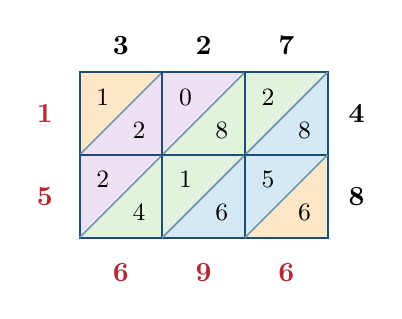
\begin{tikzpicture}[scale=1.05]
        \lband{3}{2}{4}{bandA}\lband{3}{2}{3}{bandB}
        \lband{3}{2}{2}{bandC}\lband{3}{2}{1}{bandD}
        \lband{3}{2}{0}{bandA}
        \lgrid{3}{2}
        \ltop{1}{3}\ltop{2}{2}\ltop{3}{7}
        \lside{3}{1}{4}\lside{3}{2}{8}
        \lcell{1}{1}{1}{2}\lcell{2}{1}{0}{8}\lcell{3}{1}{2}{8}
        \lcell{1}{2}{2}{4}\lcell{2}{2}{1}{6}\lcell{3}{2}{5}{6}
        \lleft{1}{1}\lleft{2}{5}
        \lbot{3}{2}{1}{6}\lbot{3}{2}{2}{9}\lbot{3}{2}{3}{6}
      \end{tikzpicture}
    \end{column}
    \begin{column}{0.5\textwidth}
      \begin{center}\small
      \begin{tabular}{lll}
        units       & $6$                & $=6$\\
        tens        & $5+6+8$            & $=19$ \hl{$\to$ 9, carry 1}\\
        hundreds    & $1+4+2+8+\hl{1}$   & $=16$ \hl{$\to$ 6, carry 1}\\
        thousands   & $2+0+2+\hl{1}$     & $=5$\\
        ten thous.  & $1$                & $=1$\\
      \end{tabular}
      \end{center}
      \vspace{4pt}
      \begin{itemize}
        \item Three digits by two digits $\Rightarrow$ a $3\times 2$ lattice.
        \item Nothing else changes.
        \item \large $327\times48 = \hl{15\,696}$
      \end{itemize}
      \vspace{2pt}
    \end{column}
  \end{columns}
\end{frame}

%=====================================================================
\begin{frame}{Your turn: lattice}
  \begin{center}
    \begin{tabular}{lll}
      \textbf{(a)} $38\times 24 = \ablank{912}$ &\quad
      \textbf{(b)} $65\times 43 = \ablank{2795}$ &\quad
      \textbf{(c)} $57\times 89 = \ablank{5073}$\\[10pt]
      \textbf{(d)} $127\times 36 = \ablank{4572}$ &\quad
      \textbf{(e)} $408\times 57 = \ablank{23\,256}$ &\quad
      \textbf{(f)} $234\times 156 = \ablank{36\,504}$
    \end{tabular}
  \end{center}
  \vspace{14pt}
  \begin{center}
    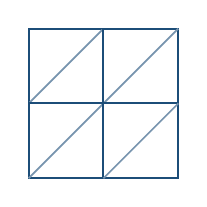
\begin{tikzpicture}[scale=0.95]
      \lgrid{2}{2}
    \end{tikzpicture}
    \hspace{26pt}
    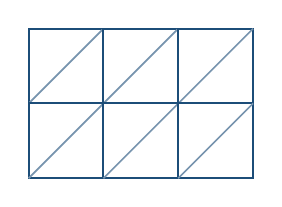
\begin{tikzpicture}[scale=0.95]
      \lgrid{3}{2}
    \end{tikzpicture}
    \hspace{26pt}
    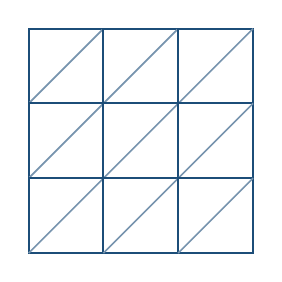
\begin{tikzpicture}[scale=0.95]
      \lgrid{3}{3}
    \end{tikzpicture}
  \end{center}
\end{frame}

%=====================================================================
\begin{frame}[plain]
  \vfill
  \centering
  {\Huge\bfseries\color{mmblue} And now the decimal point}\\
\end{frame}

%=====================================================================
\begin{frame}{First: always estimate}
  \begin{center}
    \Large $4.7 \times 3.6$
  \end{center}
  \vspace{4pt}
  \begin{center}
    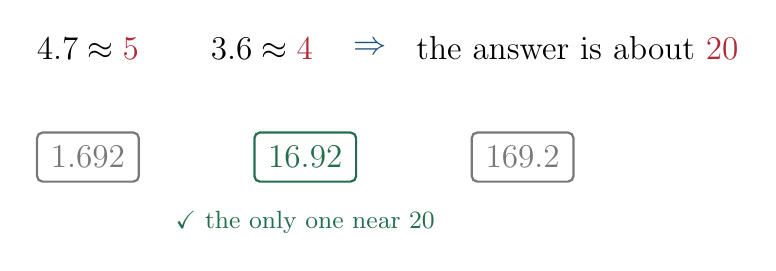
\begin{tikzpicture}[scale=0.92]
      \node[font=\large] at (0,0) {$4.7 \approx \hl{5}$};
      \node[font=\large] at (2.4,0) {$3.6 \approx \hl{4}$};
      \node[font=\large] at (3.9,0) {\textcolor{mmblue}{$\Rightarrow$}};
      \node[font=\large,anchor=west] at (4.4,0) {the answer is about $\hl{20}$};
      \foreach \x/\lab/\col in {0/$1.692$/mmgrey, 3/$16.92$/mmgreen, 6/$169.2$/mmgrey}
        {\node[draw=\col,thick,rounded corners=2pt,inner sep=5pt,text=\col,font=\large]
           at (\x,-1.5) {\lab};}
      \node[mmgreen,font=\small] at (3,-2.4) {\checkmark\ the only one near $20$};
    \end{tikzpicture}
  \end{center}
  \vspace{2pt}
  \begin{itemize}
    \item The lattice will give the digits $1\,6\,9\,2$ whatever the decimal points
          are doing.
    \item We just need to work out where the decimal point goes.
  \end{itemize}
\end{frame}

%=====================================================================
\begin{frame}{The decimal point rule}
  \begin{columns}[c]
    \begin{column}{0.5\textwidth}
      \centering
      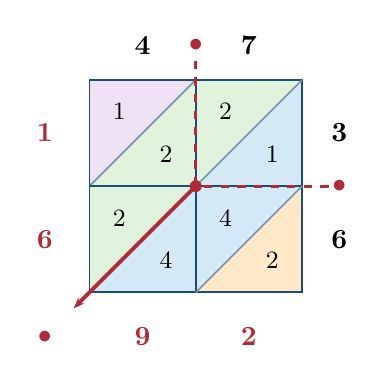
\begin{tikzpicture}[scale=1.35]
        \lband{2}{2}{3}{bandA}\lband{2}{2}{2}{bandB}
        \lband{2}{2}{1}{bandC}\lband{2}{2}{0}{bandD}
        \lgrid{2}{2}
        \ltop{1}{4}\ltop{2}{7}\lside{2}{1}{3}\lside{2}{2}{6}
        \lcell{1}{1}{1}{2}\lcell{2}{1}{2}{1}
        \lcell{1}{2}{2}{4}\lcell{2}{2}{4}{2}
        % decimal markers
        \node[mmred,font=\bfseries] at (1,0.32) {$\bullet$};
        \node[mmred,font=\bfseries] at (2.35,-1) {$\bullet$};
        \draw[mmred,dashed,line width=1pt] (1,0.18) -- (1,-1);
        \draw[mmred,dashed,line width=1pt] (2.25,-1) -- (1,-1);
        \fill[mmred] (1,-1) circle (1.6pt);
        \draw[mmred,line width=1.4pt,-{Stealth[length=4pt]}] (1,-1) -- (-0.15,-2.15);
        \lleft{1}{1}\lleft{2}{6}
        \lbot{2}{2}{1}{9}\lbot{2}{2}{2}{2}
        \node[mmred,font=\bfseries] at (-0.42,-2.42) {$\bullet$};
      \end{tikzpicture}
    \end{column}
    \begin{column}{0.5\textwidth}
      \begin{enumerate}
        \item Ignore the decimal points and build the lattice from the
              \textbf{digits}: $47$ and $36$.
        \item Mark the decimal point of the top number on the \textbf{top edge},
              and of the side number on the \textbf{right edge}.
        \item Slide one \emph{down} and the other \emph{across} until they
              \hl{meet}.
        \item From that meeting point, \hl{follow the diagonal} down-left until you
              leave the lattice. That is where the decimal point goes in the answer.
      \end{enumerate}
      \vspace{6pt}
      \begin{center}\large $4.7\times 3.6 = \hl{16.92}$\end{center}
      {\color{mmgrey}\small Estimate was $20$. \gd{\checkmark}}
    \end{column}
  \end{columns}
\end{frame}

%=====================================================================
\begin{frame}{Same lattice, different decimal point}
  \begin{columns}[c]
    \begin{column}{0.5\textwidth}
      \centering
      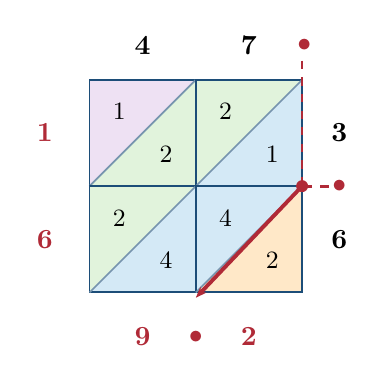
\begin{tikzpicture}[scale=1.35]
        \lband{2}{2}{3}{bandA}\lband{2}{2}{2}{bandB}
        \lband{2}{2}{1}{bandC}\lband{2}{2}{0}{bandD}
        \lgrid{2}{2}
        \ltop{1}{4}\ltop{2}{7}\lside{2}{1}{3}\lside{2}{2}{6}
        \lcell{1}{1}{1}{2}\lcell{2}{1}{2}{1}
        \lcell{1}{2}{2}{4}\lcell{2}{2}{4}{2}
        \node[mmred,font=\bfseries] at (2.02,0.32) {$\bullet$};
        \node[mmred,font=\bfseries] at (2.35,-1) {$\bullet$};
        \draw[mmred,dashed,line width=1pt] (2,0.18) -- (2,-1);
        \draw[mmred,dashed,line width=1pt] (2.25,-1) -- (2,-1);
        \fill[mmred] (2,-1) circle (1.6pt);
        \draw[mmred,line width=1.4pt,-{Stealth[length=4pt]}] (2,-1) -- (1,-2.05);
        \lleft{1}{1}\lleft{2}{6}
        \lbot{2}{2}{1}{9}\lbot{2}{2}{2}{2}
        \node[mmred,font=\bfseries] at (1,-2.42) {$\bullet$};
      \end{tikzpicture}
    \end{column}
    \begin{column}{0.5\textwidth}
      \begin{center}\Large $47 \times 3.6$\end{center}
      \vspace{4pt}
      \begin{itemize}
        \item $47$ has no decimal point written, so it sits at the
              \textbf{far right} of the top edge.
        \item $3.6$ puts its point between the two rows, as before.
        \item They meet lower down, so the diagonal leaves the lattice one place
              further right.
      \end{itemize}
      \vspace{6pt}
      \begin{center}\large $47\times 3.6 = \hl{169.2}$\end{center}
      \vspace{4pt}
      {\color{mmgrey}\small Estimate: $50\times 4 = 200$. \gd{\checkmark}\\
       The lattice digits never changed: $1\,6\,9\,2$. Only the point moved.}
    \end{column}
  \end{columns}
\end{frame}

%=====================================================================
\begin{frame}{The quick check: count the decimal places}
  \begin{center}
    \begin{tabular}{lcl}
      $4.7\times 3.6$  & $1+1 = 2$ places & $\Rightarrow$ $16\hl{.}92$\\
      $47\times 3.6$   & $0+1 = 1$ place  & $\Rightarrow$ $169\hl{.}2$\\
      $0.47\times 3.6$ & $2+1 = 3$ places & $\Rightarrow$ $1\hl{.}692$\\
      $0.47\times 0.36$& $2+2 = 4$ places & $\Rightarrow$ $0\hl{.}1692$\\
    \end{tabular}
  \end{center}
  \vspace{10pt}
  \begin{itemize}
    \item The digits $1692$ come from the same lattice every single time.
    \item Total decimal places in the question $=$ decimal places in the answer.
    \item The diagonal rule and the counting rule always agree --- use whichever
          you prefer, and \emph{check against your estimate}.
  \end{itemize}
  \vspace{6pt}
  {\color{mmgrey}\small Careful with (d): after counting four places you need a
   leading zero to fill the gap.}
\end{frame}

%=====================================================================
\begin{frame}{Worked example: $12.5 \times 3.4$}
  \begin{columns}[c]
    \begin{column}{0.5\textwidth}
      \centering
      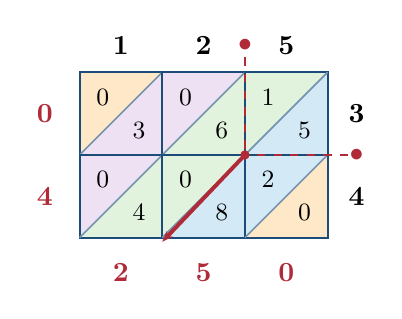
\begin{tikzpicture}[scale=1.05]
        \lband{3}{2}{4}{bandA}\lband{3}{2}{3}{bandB}
        \lband{3}{2}{2}{bandC}\lband{3}{2}{1}{bandD}
        \lband{3}{2}{0}{bandA}
        \lgrid{3}{2}
        \ltop{1}{1}\ltop{2}{2}\ltop{3}{5}
        \lside{3}{1}{3}\lside{3}{2}{4}
        \lcell{1}{1}{0}{3}\lcell{2}{1}{0}{6}\lcell{3}{1}{1}{5}
        \lcell{1}{2}{0}{4}\lcell{2}{2}{0}{8}\lcell{3}{2}{2}{0}
        \node[mmred,font=\bfseries] at (2,0.32) {$\bullet$};
        \node[mmred,font=\bfseries] at (3.35,-1) {$\bullet$};
        \draw[mmred,dashed,line width=1pt] (2,0.18) -- (2,-1);
        \draw[mmred,dashed,line width=1pt] (3.25,-1) -- (2,-1);
        \fill[mmred] (2,-1) circle (1.6pt);
        \draw[mmred,line width=1.4pt,-{Stealth[length=4pt]}] (2,-1) -- (1,-2.05);
        \lleft{1}{0}\lleft{2}{4}
        \lbot{3}{2}{1}{2}\lbot{3}{2}{2}{5}\lbot{3}{2}{3}{0}
      \end{tikzpicture}
    \end{column}
    \begin{column}{0.5\textwidth}
      \begin{center}\small
      \begin{tabular}{lll}
        units      & $0$                & $=0$\\
        tens       & $2+8+5$            & $=15$ \hl{$\to$ 5, carry 1}\\
        hundreds   & $0+4+1+6+\hl{1}$   & $=12$ \hl{$\to$ 2, carry 1}\\
        thousands  & $0+0+3+\hl{1}$     & $=4$\\
        ten thous. & $0$                & $=0$\\
      \end{tabular}
      \end{center}
      \vspace{6pt}
      \begin{itemize}
        \item Digits: $125\times 34 = 4250$.
        \item Points meet after the $2$ on top and between the rows, so the diagonal
              exits one place from the right.
        \item \large $12.5\times 3.4 = \hl{42.50} = \hl{42.5}$
      \end{itemize}
      \vspace{2pt}
      {\color{mmgrey}\scriptsize Estimate: $13\times 3 \approx 39$. \gd{\checkmark}
       A trailing zero after the point can be dropped.}
    \end{column}
  \end{columns}
\end{frame}

%=====================================================================
\begin{frame}{Your turn: decimals}
  \begin{center}
    \begin{tabular}{lll}
      \textbf{(a)} $2.4\times 3.7 = \ablank{8.88}$ &\quad
      \textbf{(b)} $6.3\times 0.8 = \ablank{5.04}$ &\quad
      \textbf{(c)} $5.2\times 4.6 = \ablank{23.92}$\\[10pt]
      \textbf{(d)} $0.46\times 2.3 = \ablank{1.058}$ &\quad
      \textbf{(e)} $13.4\times 2.5 = \ablank{33.5}$ &\quad
      \textbf{(f)} $0.85\times 0.64 = \ablank{0.544}$
    \end{tabular}
  \end{center}
  \vspace{10pt}
  \begin{center}
    \begin{minipage}{0.86\textwidth}
      \small
      \textbf{For each one, write your estimate before you start.}\\[8pt]
      \textbf{Challenge 1.} $1.25\times 0.48$. Why does the answer need fewer
      digits than you expect? \quad \ablank{$=0.6$; the lattice gives $6000$ and
      the trailing zeros disappear.}\\[6pt]
      \textbf{Challenge 2.} A lattice for $\square.\square \times 4.5$ gives the
      digits $2\,7\,9\,0$ and the answer $27.90$. What was the first number?
      \quad \ablank{$6.2$}\\[6pt]
      \textbf{Challenge 3.} Explain to your partner why a diagonal is the same
      thing as a place-value column.
    \end{minipage}
  \end{center}
\end{frame}

%=====================================================================
\begin{frame}{Summary}
  \begin{columns}[T]
    \begin{column}{0.32\textwidth}
      \centering
      {\color{mmblue}\bfseries Area}\\[4pt]
      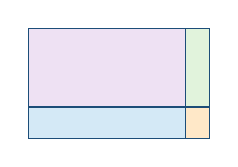
\begin{tikzpicture}[scale=0.1]
        \fill[bandD] (0,4) rectangle (20,14);\fill[bandC] (20,4) rectangle (23,14);
        \fill[bandB] (0,0) rectangle (20,4);\fill[bandA] (20,0) rectangle (23,4);
        \draw[mmblue] (0,0) rectangle (23,14);
        \draw[mmblue] (20,0)--(20,14);\draw[mmblue] (0,4)--(23,4);
      \end{tikzpicture}\\[4pt]
      {\scriptsize Split each number into place values; the four areas are the four
       products.}
    \end{column}
    \begin{column}{0.32\textwidth}
      \centering
      {\color{mmblue}\bfseries Grid}\\[4pt]
      {\scriptsize\begin{tabular}{|c|c|c|}\hline
        $\times$&$40$&$7$\\\hline $30$&$1200$&$210$\\\hline $6$&$240$&$42$\\\hline
      \end{tabular}}\\[4pt]
      {\scriptsize Every zero written out. Reliable, but a long addition at the end.}
    \end{column}
    \begin{column}{0.32\textwidth}
      \centering
      {\color{mmblue}\bfseries Lattice}\\[4pt]
      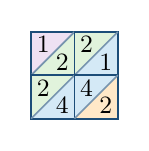
\begin{tikzpicture}[scale=0.55]
        \lband{2}{2}{3}{bandA}\lband{2}{2}{2}{bandB}
        \lband{2}{2}{1}{bandC}\lband{2}{2}{0}{bandD}
        \lgrid{2}{2}
        \lcell{1}{1}{1}{2}\lcell{2}{1}{2}{1}
        \lcell{1}{2}{2}{4}\lcell{2}{2}{4}{2}
      \end{tikzpicture}\\[4pt]
      {\scriptsize Digits only. The diagonals carry the place value. Read down,
       then across.}
    \end{column}
  \end{columns}
  \vspace{12pt}
  \begin{center}
    \begin{minipage}{0.88\textwidth}
      \begin{itemize}
        \item Tens in the upper-left triangle, units in the lower-right.
        \item Add down the diagonals from the bottom right, carrying up-left.
        \item \textbf{Decimals:} drop one point down, bring the other across, then
              follow the diagonal out. Or count the decimal places.
        \item \textbf{Always estimate first.}
      \end{itemize}
    \end{minipage}
  \end{center}
\end{frame}

\end{document}